\section{A resolved moving-threshold curve}
\label{sec:movingcurve}
We now evaluate the full limiting integral of
Section~\ref{sec:preparation}, rather than constructing a curve from its
local corner coefficient. The model remains dS$_2$, $L=1$, proper
$SO^+(2,1)$, strict $G_N\to0$, BD free matter with two independent equal
principal-series species, a normalized vacuum external packet, fixed
proper Gaussian smearing, and the repeated moving projection $Q_M$.
Here $\pi_0(r)=\beta e^{-\beta r}$. The numerical example fixes
$\nu=0.6$, $\sigma=\beta=1$. All times use
$t_M=\log(2M)+T$, with $M\to\infty$ taken first.

\subsection{Splitting every transverse boundary}
Integrating the external excess $r$ exactly gives
\begin{equation}
 J_Q(\chi)=\iint_{\mathbb R^2} f_\chi(u)f_\chi(v)
 \exp\!\left[-\beta\max\left(0,-u-\frac\chi2,
                  -v-\frac\chi2,-u-v\right)\right]\dd u\dd v.
 \label{eq:mq-weight}
\end{equation}
This is still the hard projection, with no smoothing of its boundaries.
For fixed $u$, set
\begin{align}
 a_\chi(u)&=\max(0,-u-\chi/2),&
 b_\chi(u)&=\max(-\chi/2,-u),\notag\\
 E_\chi(s)&=\int_{-\infty}^s e^{\beta v}f_\chi(v)\dd v,&
 H_\chi(s)&=\int_s^\infty f_\chi(v)\dd v.
\end{align}
The maximum in \eqref{eq:mq-weight} is
$\max(a_\chi,b_\chi-v)$. Its two branches meet at $v=b_\chi-a_\chi$, so
\begin{equation}
 J_Q(\chi)=\int f_\chi(u)
 \left[e^{-\beta b_\chi}E_\chi(b_\chi-a_\chi)
       +e^{-\beta a_\chi}H_\chi(b_\chi-a_\chi)\right]\dd u.
 \label{eq:mq-slice}
\end{equation}
The outer panels split at $u=\pm\chi/2$, and each inner panel ends at
the actual moving boundary. No tensor rule is applied across a max fold.

As an independent geometric representation, use symmetry to restrict to
$v\le u$, and put $d_\chi(u)=\chi/2$ for $u\ge\chi/2$ and
$d_\chi(u)=u$ otherwise. Then
\begin{equation}
 J_Q(\chi)=2\int f_\chi(u)\left[
 e^{\beta d_\chi(u)}E_\chi\bigl(\min(u,-d_\chi(u))\bigr)
 +\one_{u>-d_\chi(u)}\int_{-d_\chi(u)}^u f_\chi(v)\dd v
 \right]\dd u.
 \label{eq:mq-ordered}
\end{equation}
Indeed, in this half-plane $-v-\chi/2\ge-u-\chi/2$; comparison with
$-u-v$ switches at $u=\chi/2$. Both implementations retain complex
$f_\chi$. They share the same special-function routine, so agreement
checks geometry and quadrature, not independent Gamma certification.

\subsection{Static normalization and stable small differences}
At $\chi=0$, the weight factorizes. With $k(w)=f_0(w)/(16\pi^3)$, define
\begin{align}
 g&=\int_0^\infty k(x)\dd x,&
 \ell&=\int_0^\infty k(-u)e^{-\beta u}\dd u,\notag\\
 m&=\int_0^\infty\!\int_0^\infty
       k(x)k(-u)e^{-\beta(u-x)_+}\dd u\dd x.
\end{align}
The two-step path norm and early crossed plateau are
\begin{equation}
 N_\infty^Q=g^2+g\ell+m+\ell^2,\qquad
 X_\infty^Q=(g+\ell)^2,\qquad
 \mathcal D_{\rm edge}=2(m-g\ell).
 \label{eq:mq-static}
\end{equation}
The last difference is computed directly as a positive integral with
weight $e^{-\beta(u-x)_+}(1-e^{-\beta\min(u,x)})$, using
\texttt{expm1}. The resulting values are
\begin{align}
 N_\infty^Q&\simeq0.007843474197608,\notag\\
 X_\infty^Q&\simeq0.007649270098482,\notag\\
 \mathcal D_{\rm edge}&\simeq0.0003884081982512.
 \label{eq:mq-static-values}
\end{align}
The independently evaluated $J_Q(0)/(256\pi^6)$ agrees with
$X_\infty^Q$.

For either subtraction width $a=1$ or $2$, let
\begin{equation}
 I_a(T)=\int e^{iT\chi}
 \left[A_Q(\chi)-\frac{iX_\infty^Q e^{-a\chi^2}}{2\pi\chi}\right]\dd\chi.
\end{equation}
The exact representations used in the numerical calculation are
\begin{align}
 \mathcal X_Q(T)&=\frac{X_\infty^Q}{2}
       \left[1-\operatorname{erf}\!\left(\frac{T}{2\sqrt a}\right)\right]
       +I_a(T),\notag\\
 \mathcal D_Q(T)-\mathcal D_{\rm edge}
   &=X_\infty^Q\left[1+\operatorname{erf}\!\left(\frac{T}{2\sqrt a}\right)\right]
       -2\operatorname{Re}I_a(T).
 \label{eq:mq-small-difference}
\end{align}
The second line avoids subtracting two plateau-size commutators. It
does not remove cancellation inside the Fourier integral. Unlike the
fixed protocol, $\mathcal X_Q$ need not be real: for example
$\mathcal X_Q(0)\simeq0.00691324056+0.00008422460\,i$.

\subsection{Numerical comparison with the corner prediction}
Composite Gauss--Legendre integration uses a transverse box
$[-10,10]^2$ and $\chi\in[-12,12]$, with a panel break at zero.
Transverse/Fourier orders are varied separately as
$(24,40)$, $(32,40)$ and $(24,64)$. The central Fourier panels have
width $1/2$. Both PV subtraction widths, both transverse representations
at selected frequencies, and transverse radii $8,10,12$ are recorded.
Twenty-five detailed times and a 257-point central curve retain full
complex values.
The maximum changes in the 25 complex correlators are approximately
$6.14\times10^{-18}$ under transverse refinement and
$2.08\times10^{-17}$ under Fourier refinement. Relative to the real
early plateau difference or the real late correlator, the largest
observed change is $1.90\times10^{-7}$. These are empirical differences
between rules, not rigorous accuracy estimates.

The actual integrals give dimensionless ratios to the leading coefficient
of Theorem~\ref{thm:prep-moving}, defined by
\[
 R_{\rm early}(s)=\frac{(\mathcal D_Q(-s)-\mathcal D_{\rm edge})s^3}{2B},
 \qquad R_{\rm late}(s)=\frac{\operatorname{Re}\mathcal X_Q(s)s^3}{B}.
\]
\begin{center}
\begin{tabular}{rcc}
\toprule
$|T|$ & $R_{\rm early}(|T|)$ & $R_{\rm late}(|T|)$\\
\midrule
16 & 0.74636 & 1.75824\\
32 & 0.85907 & 1.16537\\
64 & 0.92589 & 1.08068\\
128 & 0.96205 & 1.03962\\
\bottomrule
\end{tabular}
\end{center}
These approach the predicted value one without a
fitted time shift. Even at $|T|=128$, finite-$T$ corrections are several
percent; the leading asymptotic is not an exact finite-time curve.
At $T=-128$ the early difference is about $1.09044\times10^{-10}$,
and the absolute regular-integrand scale divided by half that signal
is about $7.28\times10^7$. Refinement comparisons must therefore be
reported relative to this small signal, not only to $N_\infty^Q$.

For real frequencies Euler's integral gives
$|f_\chi(w)|\le\Gamma(1/4)^4e^{-\pi w-w^2}$ at the stated $\sigma=1$.
If $G$ is the integral of this envelope and $g_R$ its tail outside
$[-R,R]$, then the omitted transverse region contributes at most
$2Gg_R$ to $J_Q(\chi)$, since the projection weight is at most one.
The outer Gaussian similarly controls the omitted real-frequency tail.
The archived bound expressions are evaluated in floating point, without
outward rounding. They are separate tail bounds, not a certified total
error for the subtracted PV quadrature. Order comparisons provide
empirical numerical support for the curve and the corner prediction.

\begin{figure}[htbp]
 \centering
 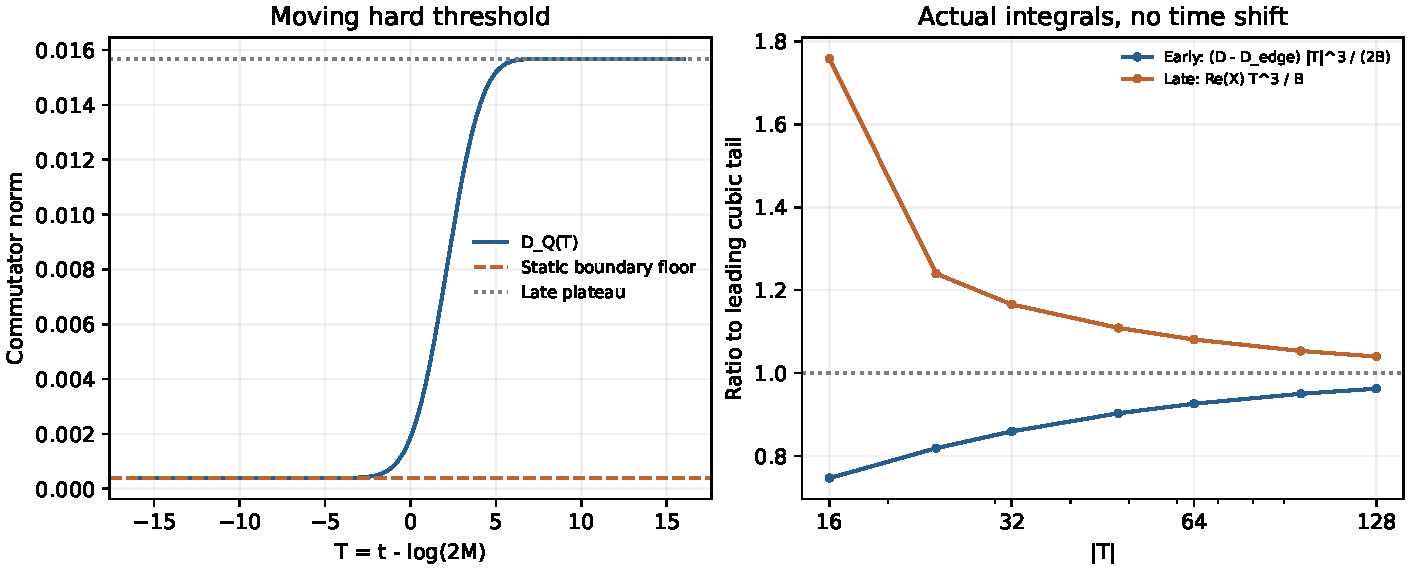
\includegraphics[width=.98\linewidth]{../results/stage3/moving-curve/moving-curve.pdf}
 \caption{Actual limiting integrals for the exponential packet and repeated
 moving hard threshold. The right panel compares independently computed
 time curves with the analytic corner coefficient; the coefficient was
 not used to generate the curves. This is ordered-limit data, not a
 finite-mass simulation or finite-$G_N$ calculation.}
 \label{fig:moving-curve}
\end{figure}
